\subsection{Akwizycja danych}
W projekcie założono wykorzystanie metod fotogrametrycznych do tworzenia trójwymiarowych modeli 
obszarów urbanistycznych. Za część projektu przyjęto z tego względu również pozyskanie własnych zestawów 
danych fotograficznych (fotogramów), które spełniałyby wymogi techniczne, umożliwiające późniejszą 
rekonstrukcję 3D. Niezbędne było wykonanie dużej liczby ujęć, obejmujących wiele kątów i perspektyw oraz 
zapewnienie odpowiedniego nakładania się zdjęć dla poprawnego działania oprogramowania fotogrametrycznego, 
które identyfikuje i dopasowuje wspólne punkty widoczne na wielu zdjęciach.

Akwizycję zrealizowano na kampusie \textbf{Politechniki Wrocławskiej}, koncentrując się na budynkach \textbf{C5}, \textbf{C7} oraz 
Strefie Kultury Studenckiej (\textbf{SKS}) \ref{fig:four-photos} i pozyskując zdjęcia zarówno z lotów bezzałogowym statkiem powietrznym, 
jak i z poziomu gruntu. Stanowią one kompletne zbiory danych, które spełniły wymogi jakościowe 
i posłużyły do budowy testowych modeli. 

\begin{figure}[h!]
    \centering
    \begin{minipage}{0.245\textwidth}
        \centering
        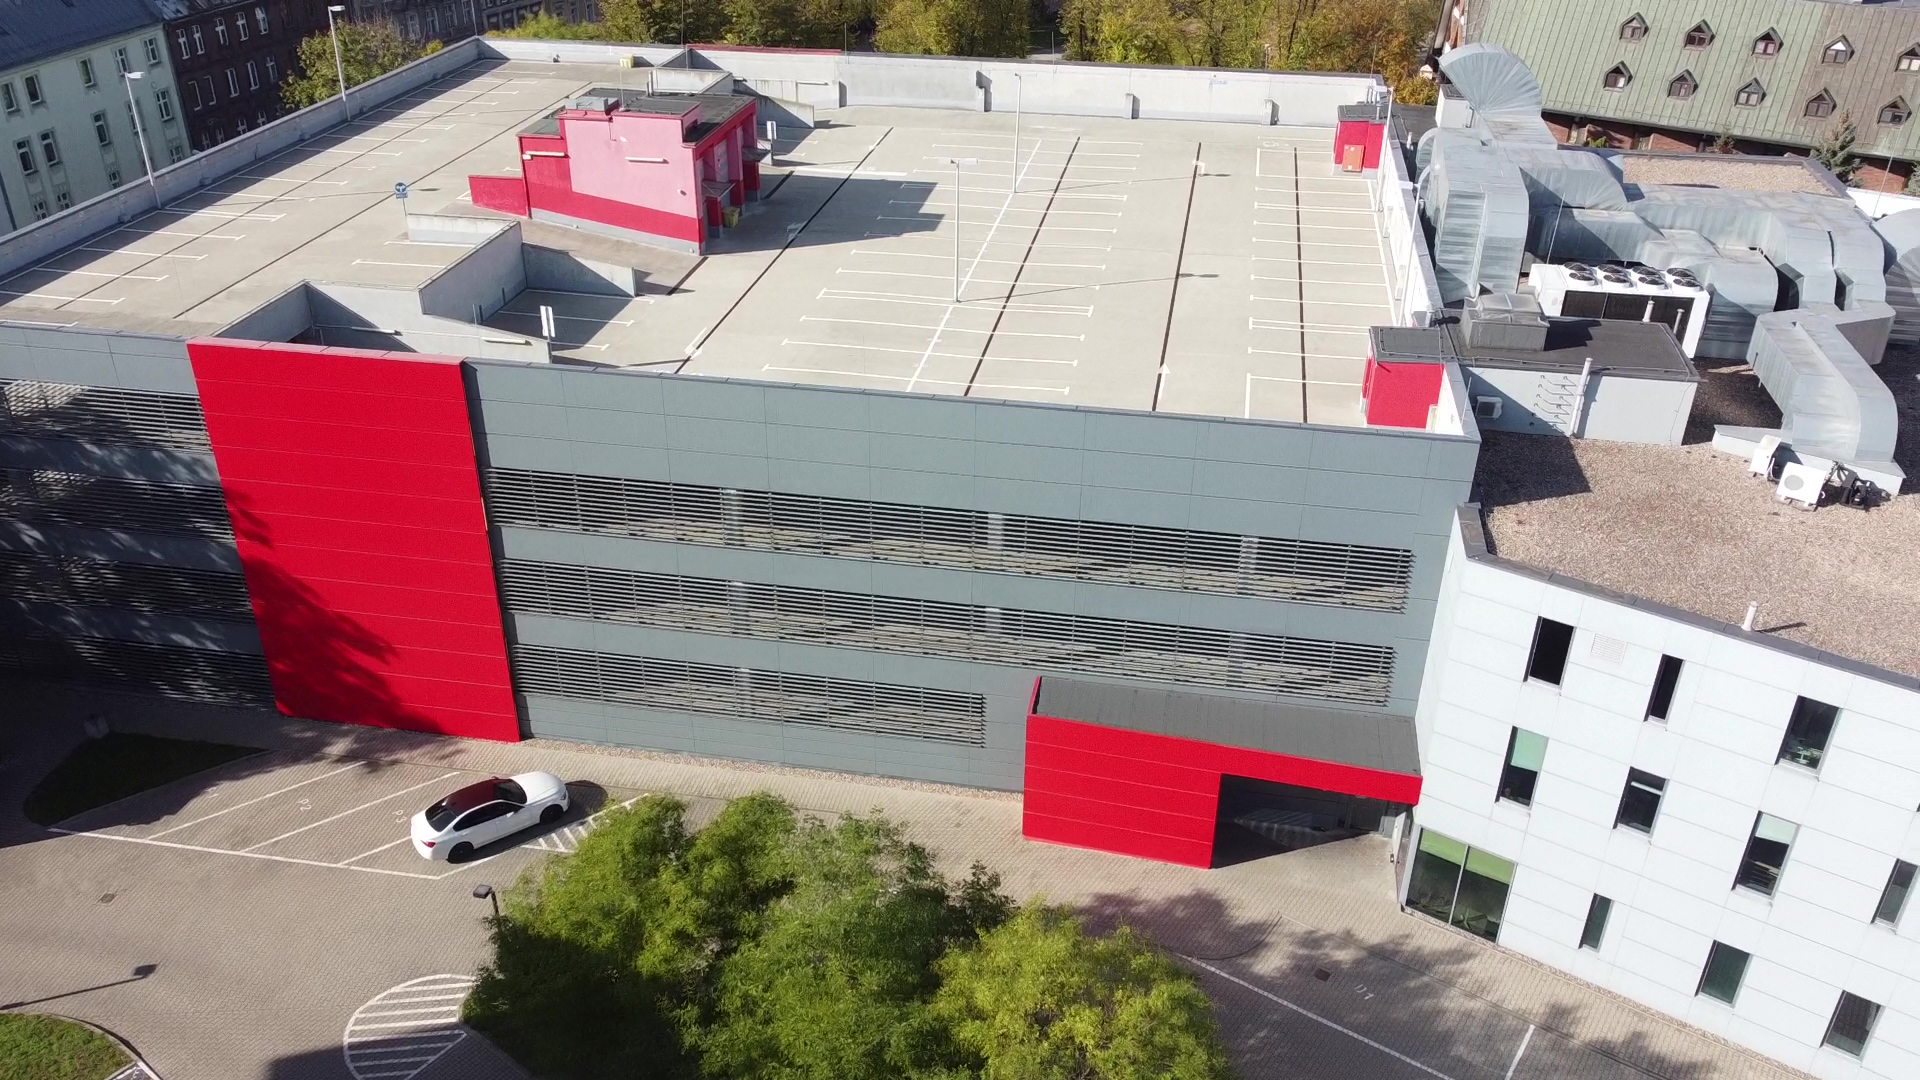
\includegraphics[width=\textwidth]{images/sks_dataset_1.jpg}
    \end{minipage}
    \hfill
    \begin{minipage}{0.245\textwidth}
        \centering
        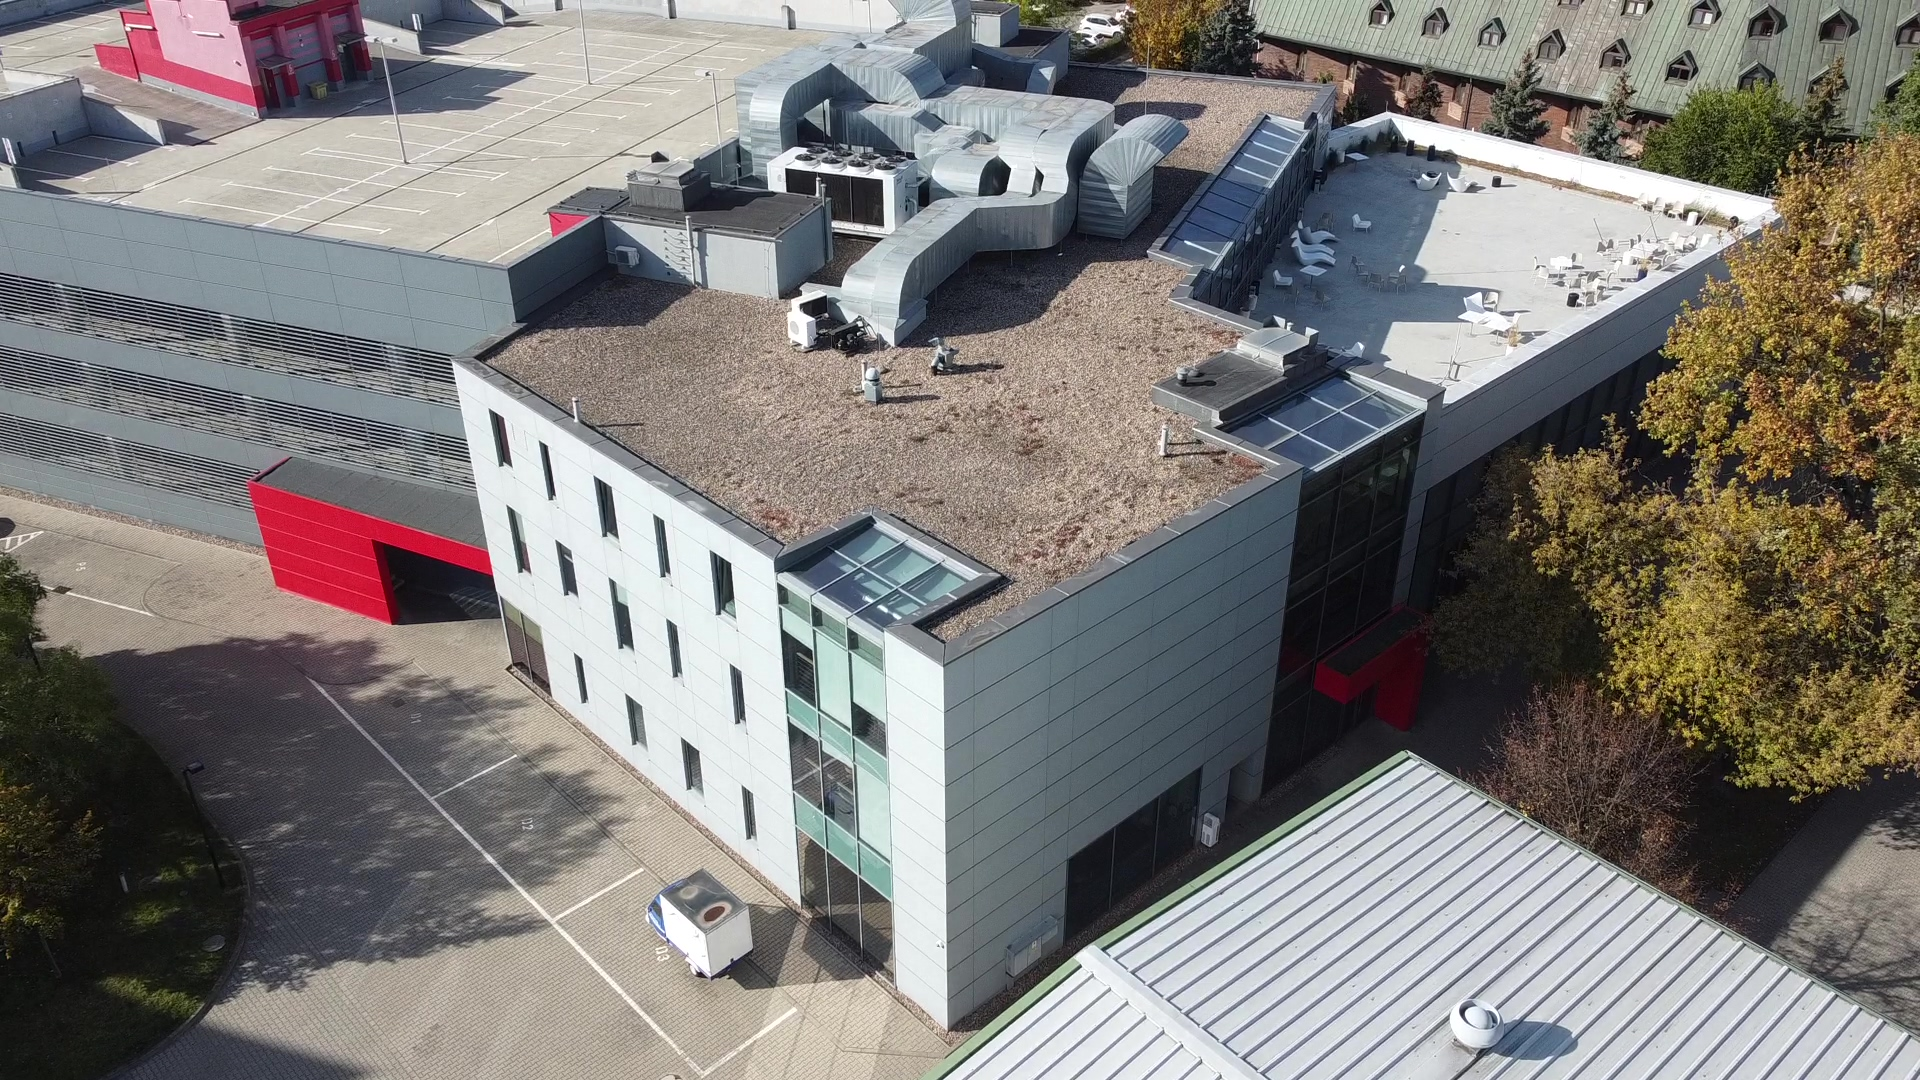
\includegraphics[width=\textwidth]{images/sks_dataset_2.jpg}
    \end{minipage}
    \hfill
    \begin{minipage}{0.245\textwidth}
        \centering
        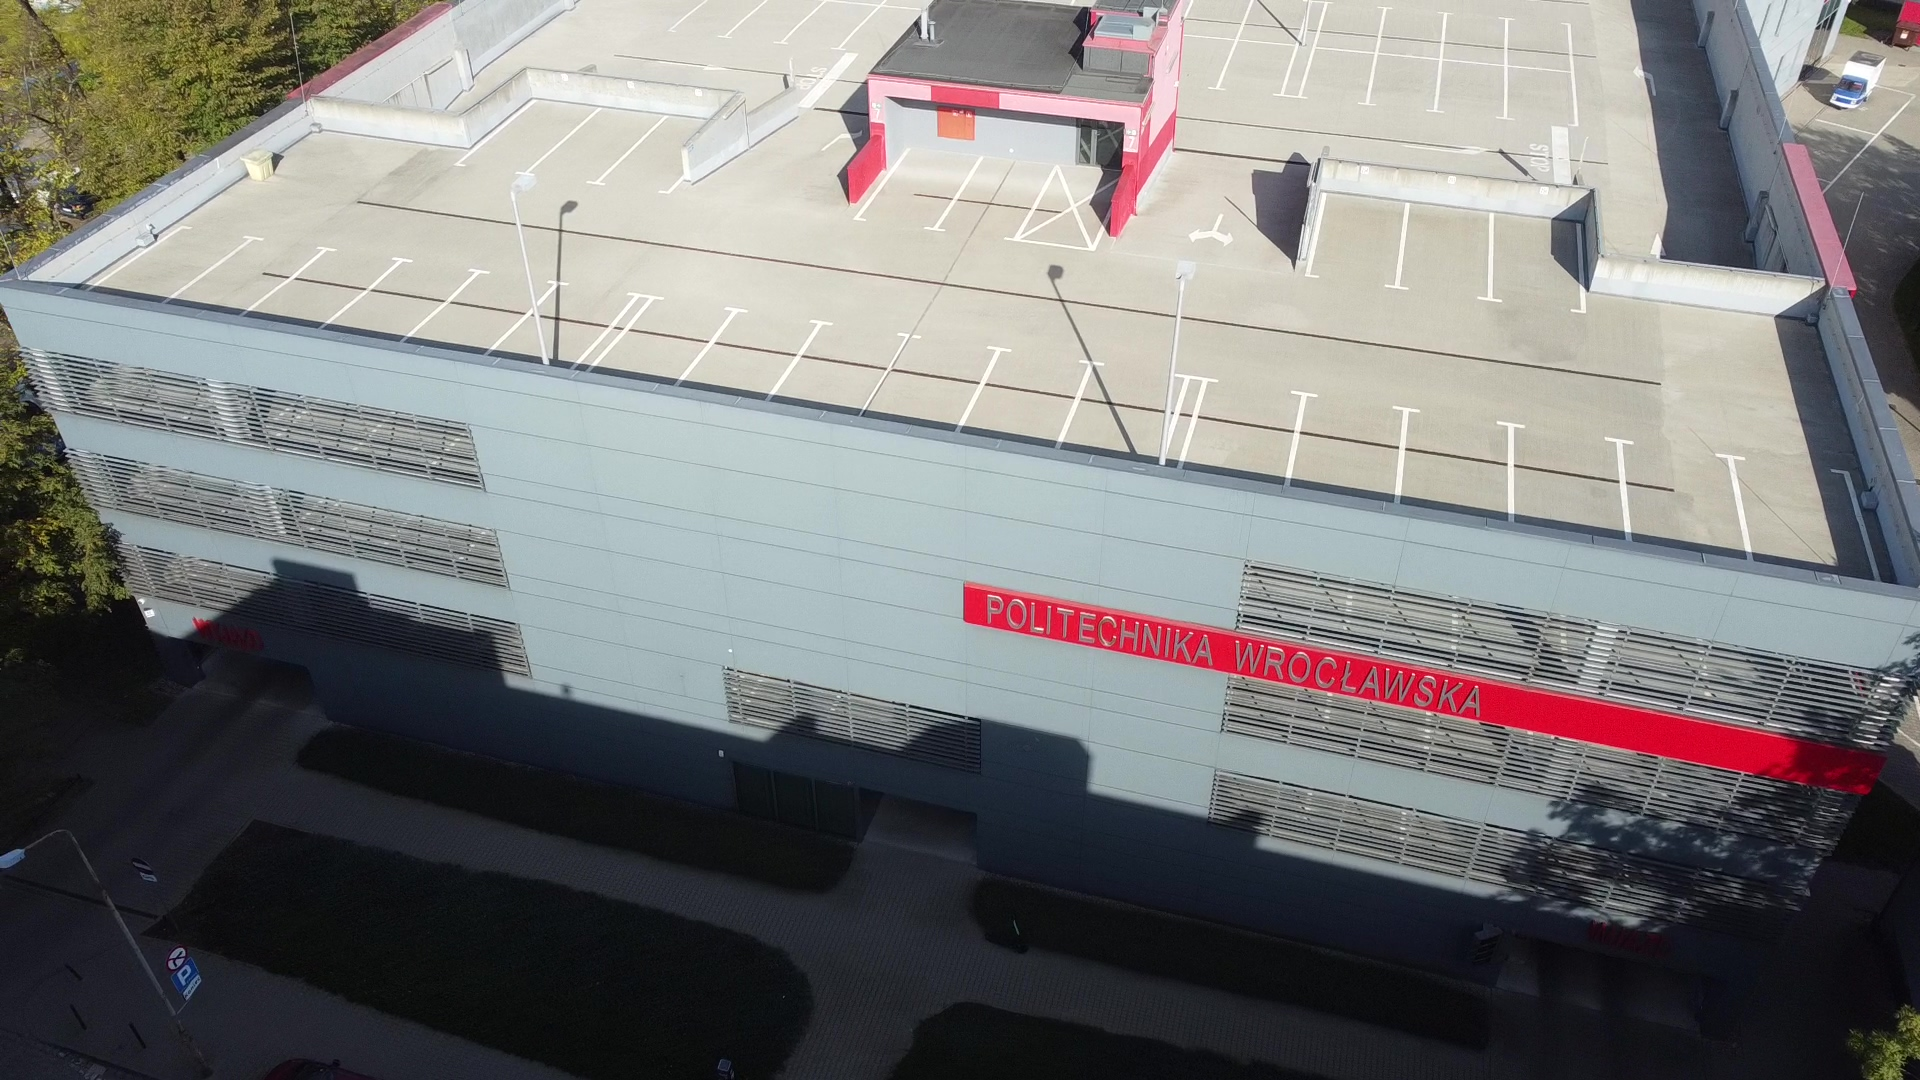
\includegraphics[width=\textwidth]{images/sks_dataset_3.jpg}
    \end{minipage}
    \hfill
    \begin{minipage}{0.245\textwidth}
        \centering
        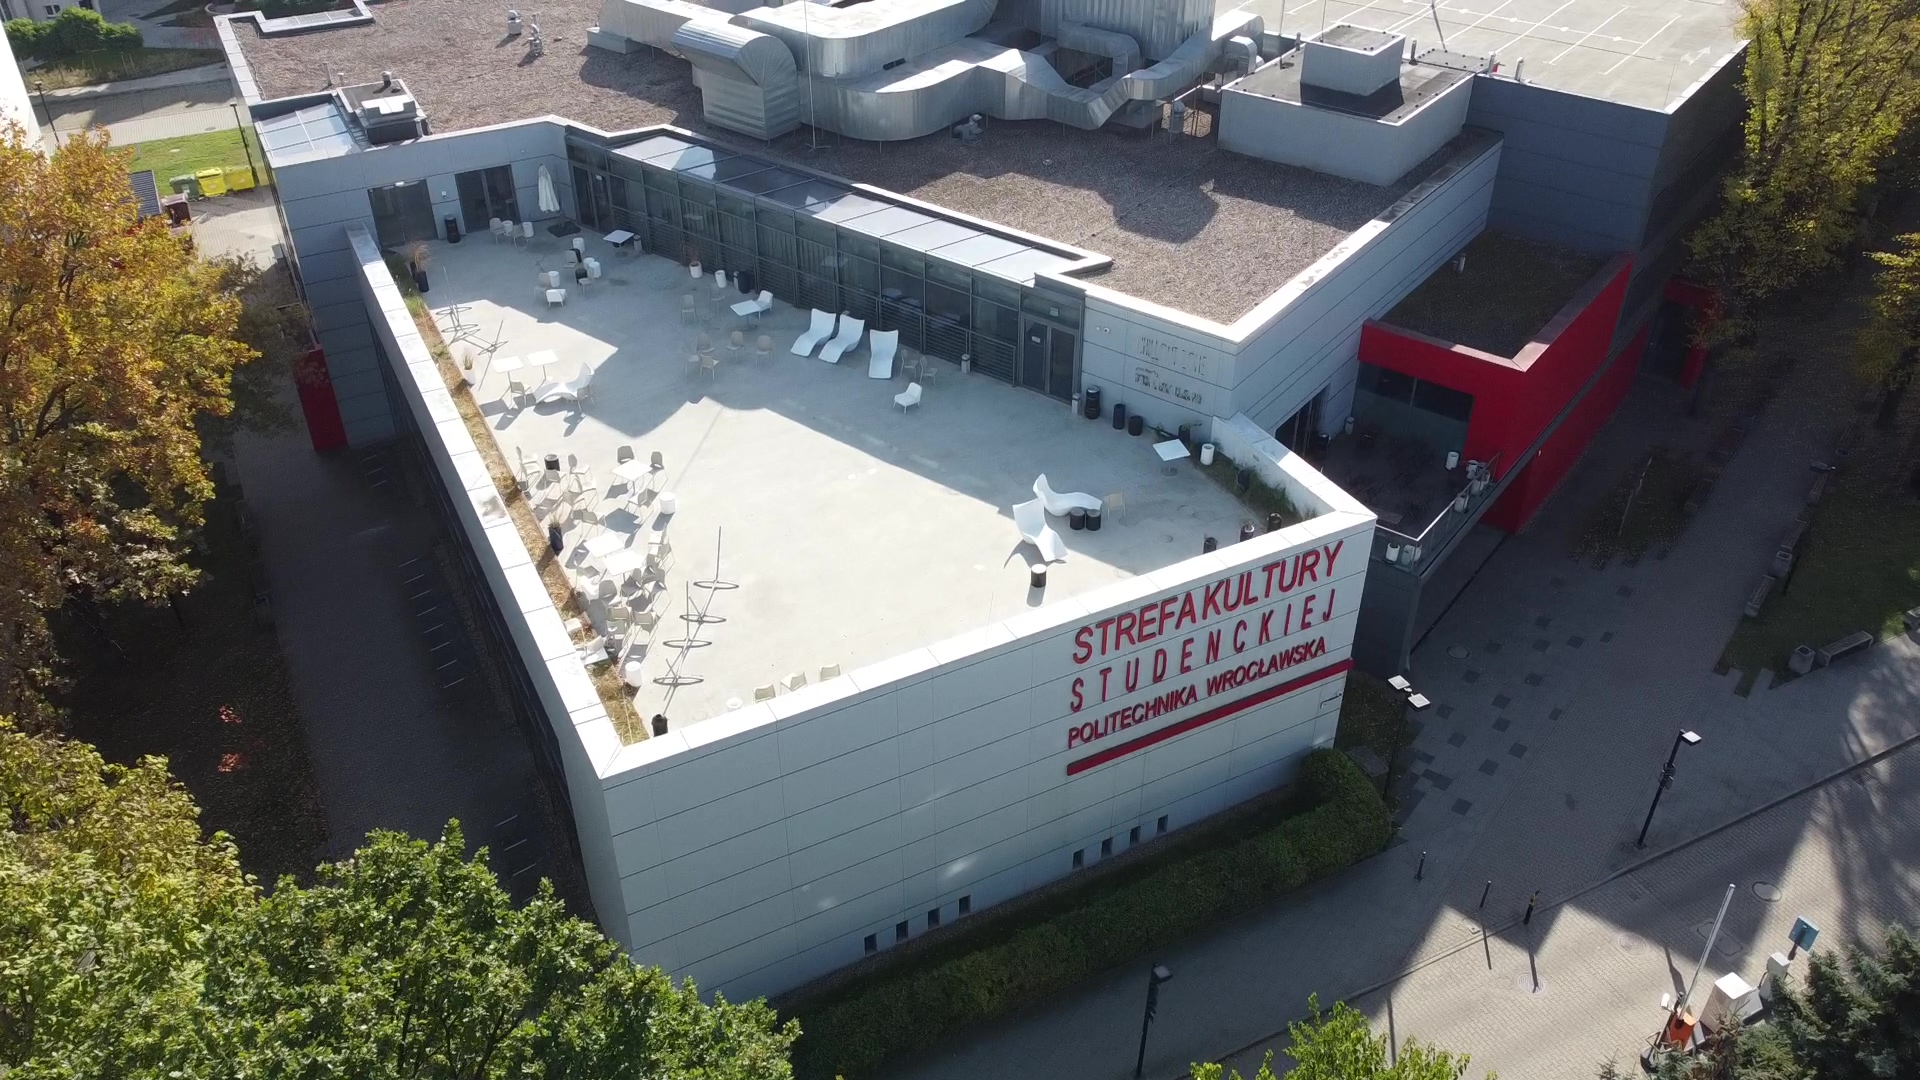
\includegraphics[width=\textwidth]{images/sks_dataset_4.jpg}
    \end{minipage}
    \caption{Przykładowe zdjęcia z akwizycji danych przedstawiające SKS}
    \label{fig:four-photos}
\end{figure}